%
% A brief introduction of evolutionary algorithm, Zhang Jiadong, 2017
%

\documentclass[12pt]{beamer}

\usetheme{metropolis}
\usepackage{appendixnumberbeamer}

\usepackage{booktabs}
\usepackage[scale=2]{ccicons}
\usepackage{listings}
\usepackage{tikz}
\usepackage[BoldFont,SlantFont,CJKchecksingle]{xeCJK}
\setCJKmainfont[BoldFont=SimHei,SlantedFont=KaiTi]{SimSun}
\setCJKsansfont[BoldFont=SimHei,SlantedFont=KaiTi]{SimSun}
\setCJKmonofont[ItalicFont={Adobe Fangsong Std}]{SimSun}
\setCJKfamilyfont{zhsong}{SimSun}
\setCJKfamilyfont{zhhei}{SimHei}
\setCJKfamilyfont{zhkai}{KaiTi}
\setCJKfamilyfont{zhfs}{FangSong}

\usepackage{pgfplots}
\usepgfplotslibrary{dateplot}

\usepackage[linesnumbered,ruled]{algorithm2e}
\usepackage{algorithmicx}
\usepackage{algpseudocode}
\usepackage{amsmath}

\usepackage{xspace}
\newcommand{\themename}{\textbf{\textsc{metropolis}}\xspace}

\title{进化算法简介}
%\subtitle{A modern beamer theme}
\date{\today}
\author{XXX XXX XXX XXX XXX XXX}
\institute{浙江大学计算机科学与技术学院}
%\titlegraphic{\hfill\includegraphics[height=1.5cm]{logo.pdf}}

\begin{document}

\maketitle

\begin{frame}{目录}
  \setbeamertemplate{section in toc}[sections numbered]
  \tableofcontents[hideallsubsections]
\end{frame}

%\section{前言}
%
%\begin{frame}[fragile]{前言}
%
%	进化算法是以达尔文的进化论思想为基础,通过模拟生物进化过程与机制的求解问题的自组织、自适应的人工智能技术。
%	
%\end{frame}

%topics

%
% GNU courseware, Zhang Jiadong, 2018
%

\section{前言}\fontsize{12pt}{12pt}\selectfont

\frame{\frametitle{定义}
又叫演化计算,是模拟自然界中的生物的演化过程产生的一种群体导向的随机搜索技术和方法。

~

是一种通用的问题求解方法,具有自组织、自适应、自学习性和本质并行性等特点,
不受搜索空间限制性条件的约束,也不需要其它辅助信息。
}

\frame{\frametitle{思想}
进化算法是受生物进化过程中“优胜劣汰”的自然选择机制和遗传信息的传递规律的影响,
通过程序迭代模拟这一过程,把要解决的问题看作环境,在一些可能的解组成的种群中,
通过自然演化寻求最优解。
}

\frame{\frametitle{种类}
	\begin{itemize}
		\item<1-> 遗传算法(Genetic Algorithms)
		\item<2-> 演化策略(Evolution Strategy)
		\item<3-> 演化规划(Evolution Programming)
		\item<4-> 遗传程序设计(Genetic Programming)
		\item<5-> 多种群协同进化(Coevolutionary Algorithm)
		\item<6-> 差分进化算法(Differential Evolutionary)
	\end{itemize}
}

%end

%
% GNU courseware, XIN YUAN, 2017
%

\section{演化规划}\fontsize{12pt}{12pt}\selectfont

%\frame{
%\centerline{\textbf{\Huge{演化规划}}}
%}

\frame{\frametitle{定义}

\begin{block}{定义}
%From Wikipedia:\\Evolutionary programming is one of the four major evolutionary algorithm paradigms. It is similar to genetic programming, but the structure of the program to be optimized is fixed, while its numerical parameters are allowed to evolve.进化规划是四种主要的演化算法之一。 它与遗传算法类似,但要优化的程序结构是固定的,而其数值参数则可以进化。
~

演化规划(Evolutionary Programming Algorithm, EPA)是由美国学者Lawrence J. Fogel于1960年提出的,它适用于解决目标函数或约束条件不可微的复杂非线性实值连续优化问题。它与遗传算法类似,但要优化的程序结构是固定的,而其数值参数则可以进化。
\end{block}
}
\begin{algorithm}
\caption{Evolutionary Programming Algorithm}
    \KwIn{个体表现型$X$, 群体规模$N$, 迭代次数$G$等}
    \KwOut{子代}
    	随机产生初始群体并计算适应值(含$N$个个体)\\
        \While{not done}{
        //终止条件:达到规定的进化代数,或若干代内种群中最好个体的函数值不再发生变化,则终止进化\\
        	\For{$\rm i = 1;i < N; i++$}
        	{
           		对$X_i$进行变异得到$X_i'$\\
				对$X_i$进行可行性检查\\
				计算$X_i$的适应值\\

        	}
        	从$2N$个个体中选择$N$个个体 //随机型q-竞争法\\
        }
        return 子代\;
\end{algorithm}
\frame{\frametitle{思想}
EP模拟生物种群层次上的进化,因此在进化过程中主要强调生物种群行为上的联系,即强调种群层次上的行为进化而建立父、子代间的行为链。
~

EP算法最重要的一个操作是变异操作。通过变异,父代群体中的每一个个体产生一个子代个体,父代和子代中最好的那一半被选择生存下来。
}

\frame{\frametitle{q-竞争选择算法}
演化规划算法的选择策略采用的是q-竞争机制,这也是与进化策略算法最大的不同点,q-竞争说白了就是选择优质解的同时,以一定的随机概率接受较差的解。多数是优解,少数是比较差的解,共同组成一组父代,为下一次进化做准备。
}

\frame{\frametitle{q-竞争选择算法}
\textbf{思想}\\
将N个父代进化的N个子代一起放在一起,从中随机选择不重复q个个体组成一个组,然后依次对2N个个体的每一个个体进行计分,将2N个依次每次一个与随机挑选出的群组的每一个成员进行比较,相比优的话,则会对应的个体的分数加1,最后对分数进行排序,选择分数最高的N个个体!
}

\frame{\frametitle{缺点}
	大量的研究证明,由于过度选择、变异操作破坏有效模式、参数选取不当等原因,该算法存在一些亟待克服
的\textbf{缺点}:\\
(1)容易出现早熟收敛现象\\
(2)进化后期,个体之间的竞争趋缓导致算法后期的搜索效率降低等。
}

\frame{\frametitle{改进}
	\begin{itemize}
		\item<1-> 基于柯西变异的进化规划算法 1996
		% 该算法能够较好地克服早熟收敛现象,但是后期搜索的效率很低
		\item<2-> 基于Lévy概率分布的进化规划算法(LEP) 2004
		% 在该算法中使用Lévy分布变异算子代替高斯分布变异算子,其思想是使用具有更大方差的变异算子来促使种群更快地收敛到最优解,但编制Lévy 算子较为困难,且使用大方差的变异算子使种群收敛到最优解的速度变慢。
		\item<3-> 一种求解数值优化问题的快速进化规划算法 2004
		% 在该算法中,对变异算子进行了改进,对成功的变异进行适当延伸,当个体变异失败时,对变异量实施Gauss或Cauchy扰动,其思想是利用高斯变异算子良好的局部搜索能力和柯西变异算子良好的全局探索能力,以期能快速收敛到最优解。但是同时使用两种变异方式,导致算法的计算复杂度增加,算法的收敛速度受到影响
		\item<4-> ... 
	\end{itemize}
}

%end

%
% GNU courseware, Zhang Jiadong, 2018
%

\section{差分进化}\fontsize{12pt}{12pt}\selectfont

\subsection{定义}
\begin{frame}{定义}
	{\bf差分进化}是一种基于群体智能的全局优化方法,其主要通过种群内个体之间的协同合作
		和相互竞争来产生群体智能,进一步指导进化过程的全局搜索。
\end{frame}

\subsection{算法思想}
\begin{frame}{算法思想}
	\begin{figure}
		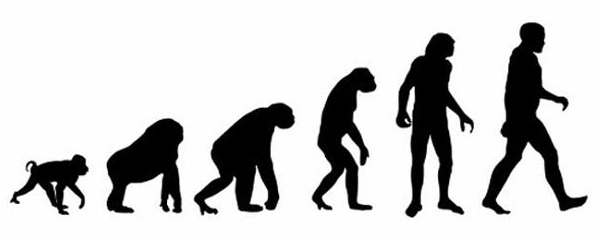
\includegraphics [width =1.0\textwidth]{../images/evolution.png}
	\end{figure}
	通过种群之间的\textbf{个体差异}和\textbf{优胜劣汰}的竞争策略产生新的个体,最终使种群接近或达到全局最优解。
\end{frame}

\subsection{算法框架}
\begin{frame}{算法框架}\small
	\begin{figure}
		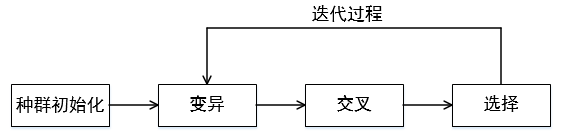
\includegraphics [width =1.0\textwidth]{../images/framework.png}
		\vspace{-1.2cm}
	\end{figure}
	\begin{itemize}
		\item {\bf 种群初始化}在解空间中随机、均匀地产生$M$个个体,每个个体由$n$个染色体组成,作为第$0$代种群,标记为
		\begin{equation*}
			\begin{split}
				X_i(0)=&\left(x_{i,1}(0),x_{i,2}(0),\cdots,x_{i,n}(0)\right)\\
				& i=1,2,\cdots,M
			\end{split}
		\end{equation*}
		\item {\bf 变异、交叉、选择 }三步操作迭代执行,直到算法收敛。第$g$次迭代的第$i$个个体标记为
		\begin{equation*}
			\begin{split}
				X_i(g)=&\left(x_{i,1}(g),x_{i,2}(g),\cdots,x_{i,n}(g)\right)\\
				& i=1,2,\cdots,M
			\end{split}
		\end{equation*}
	\end{itemize}
\end{frame}

\begin{frame}{种群初始化}
	在$n$维空间里随机产生满足约束条件的$M$个染色体,第$i$个染色体的第$j$个维取值方式如下(rand(0,1)产生0到1的均匀分布的随机数) :
	\begin{equation*}
		\begin{split}
			x_{i,j}(0) &= L_j + rand(0,1)\left(U_j-L_j\right)\\
			& i = 1,2,\cdots,M\\
			& j = 1,2,\cdots,n\\
		\end{split}
	\end{equation*}
\end{frame}

\begin{frame}{变异算子}
	在第$g$次迭代中,对个体$X_i(g)=\left(x_{i,1}(g),x_{i,2}(g),\cdots,x_{i,n}(g)\right)$,从种群中随机选择$3$个个体 $X_{p1}(g),X_{p2}(g),X_{p3}(g)$,且$ p1 \neq p2 \neq p3\neq i$, 则
	$$H_{i}(g) = X_{p1}(g)+ F\cdot\left(X_{p2}(g)-X_{p3}(g)\right)$$
	% 其中$\Delta_{p2,p3}(g)=X_{p2}(g)-X_{p3}(g)$是差分向量;$F$是缩放因子,用于控制差分向量的影响力.
	\begin{figure}
		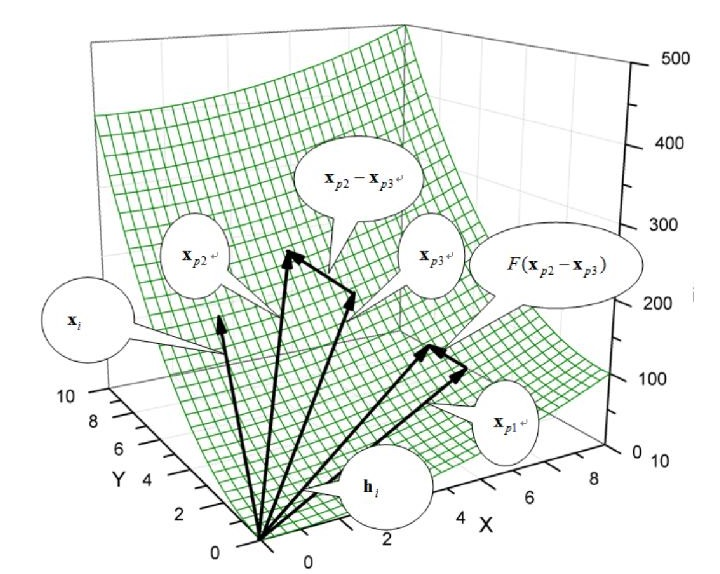
\includegraphics [width =0.55\textwidth]{../images/mutation.png}
	\end{figure}
\end{frame}

\begin{frame}{交叉算子}
	交叉操作可以增加种群的多样性,方法如下:
	$$
	v_{i,j}(g)=
	\begin{cases}
	h_{i,j}(g), rand(0,1)\le cr\\
	x_{i,j}(g), else
	\end{cases}
	$$
	其中$cr\in[0,1]$为交叉概率,$rand(0,1)$是$[0,1]$上服从均匀分布的随机数。

	\begin{figure}
		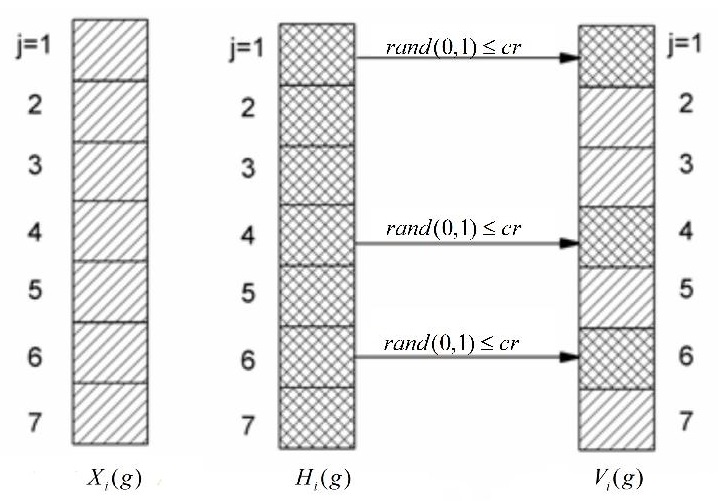
\includegraphics [width =0.55\textwidth]{../images/cross.png}
	\end{figure}
\end{frame}

\begin{frame}{选择算子}
首先查看根据评价函数选择$V_i(g)$ 或 $X_i(g)$ 作为$X_i(g+1)$
$$
	X_i(g+1) =
	\begin{cases}
	V_i(g),\qquad \mathrm{if} \quad f(V_i(g))< f(X_i(g))\\
	X_i(g),\qquad else
	\end{cases}
$$

可以看出:
	\begin{itemize}
		\item 对每个个体,$X_i(g+1)$要好于或持平$X_i(g)$。
		\item 肯定会收敛于最优点(可能是局部最优)。
		\item {\bf 变异、交叉} 操作有助于突破局部最优到达全局最优。
	\end{itemize}
\end{frame}

\subsection{应用实例}
	\begin{frame}{差分进化算法寻找函数最优解}
	定义关于参数$x, y$的函数,函数图像如左图所示
	$$f(x,y)=-20e^{-0.2\sqrt{\frac{x^2+y^2}{2}}}-e^{\frac{\cos2\pi x+\cos2\pi y}{2}}+20+e$$
	用差分进化算法求解,效果如右图所示(参数设置:$N=20, F=0.5, cr=0.5$,迭代次数 $T=300$)
	\begin{columns}
		\begin{column}{0.45\textwidth}
			\begin{figure}
				\vspace{-0.8cm}
				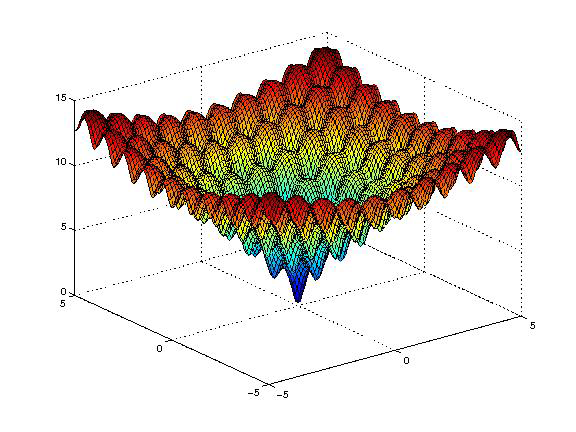
\includegraphics [width =2.0in]{../images/function.png}
			\end{figure}
		\end{column}
		\begin{column}{0.55\textwidth}
			\begin{figure}
				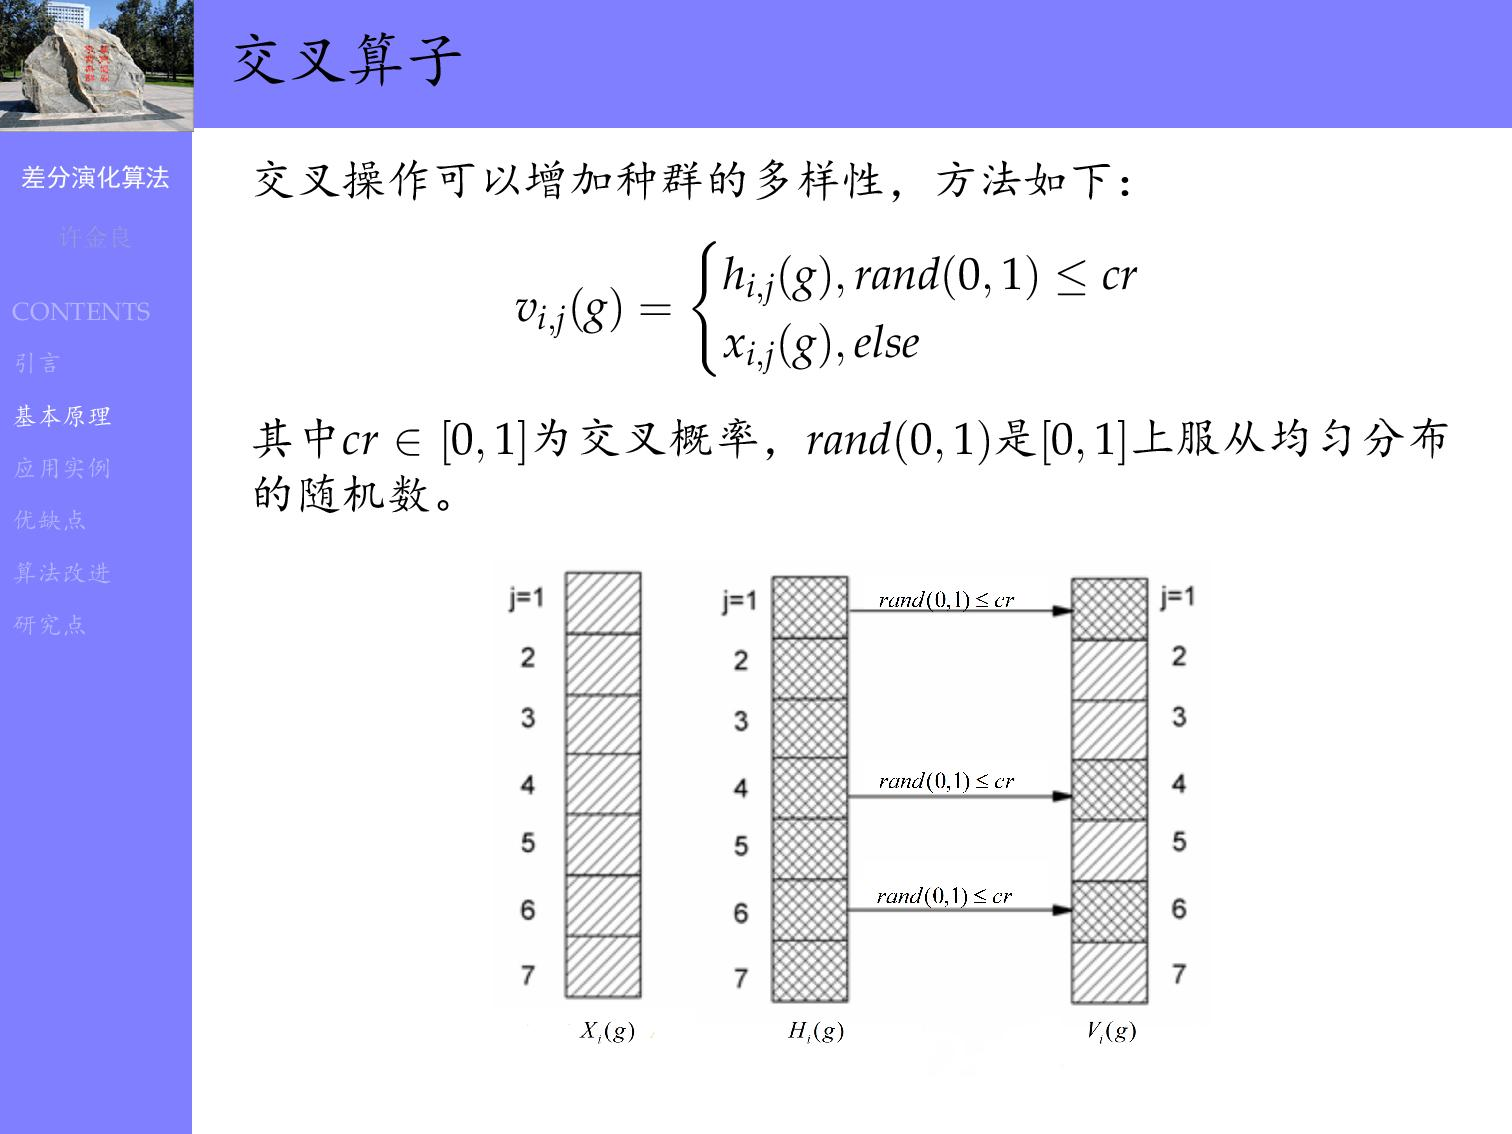
\includegraphics [width =2.0in]{../images/curve.png}
			\end{figure}
		\end{column}
	\end{columns}
\end{frame}

\subsection{优缺点}
\begin{frame}{优缺点}
和其他进化算法相比,差分进化算法具有以下优点:
	\begin{enumerate}
		\item 在非凸、多峰、非线性、连续不可微函数优化问题上表现出极强的稳健性。
		\item 收敛速度快。
		\item 操作简单,容易实现。
	\end{enumerate}
	缺点:
	\begin{enumerate}
		\item 算法后期个体间差异逐渐缩小,收敛速度慢,容易陷入局部最优。
		\item 控制参数和学习策略对算法性能有着重要的影响,并且高度依赖于优化问题的本质。
		\item 有时需要过多的迭代才能搜索到全局最优。
	\end{enumerate}
\end{frame}


\subsection{算法改进}
\subsubsection{参数控制}

\begin{frame}{参数的选取}
%参数选择主要涉及群体规模$M$,缩放因子$F$,以及交叉概率$cr$的设定\footnote{
%各研究人员得到的经验参数值往往不一致,甚至相互矛盾,所以要具体问题具体分析。}
	\begin{itemize}
		\item $M$:一般介于$5\times n$与$10\times n$之间,但不能少于$4$,否则变异算子无法进行;
		\item $F$:一般在$[0,2]$之间选择,通常取$0.5$;
		\item $cr$:一般在$[0,1]$之间选择,比较好的选择应在$0.3$左右。$cr$取值偏大,收敛速度会加快,但易发生早熟现象。
	\end{itemize}
\end{frame}

\begin{frame}{参数的自适应调整($F$)}
	将变异算子中随机选择的三个个体进行从优到劣的排序,得到$X_b,X_m,X_w$,对应适应度$f_b,f_m,f_w$,则变异算子改为:
	$$V_i=X_b+F_i\left(X_m-X_w\right)$$
	同时,$F$的取值根据生成差分向量的两个个体自适应变化,平衡全局搜索和局部搜索之间的矛盾。
	$$F_i = F_l +\left(F_u-F_l\right)\frac{f_m-f_b}{f_w-f_b}$$
	其中,$$F_l=0.1,F_u=0.9$$
\end{frame}

\begin{frame}{参数的自适应调整($cr$)}
	对于适应度好的解,取较小的$cr$,使得该解进入下一代的机会增大;
	对于适应度差的解,则取交大的$cr$,加快改变该个体的结构,使该解被淘汰掉。
	$$
	cr_i =
	\begin{cases}
		cr_l+\left(cr_u-cr_l\right)\frac{f_i-f_{min}}{f_{max}-f_{min}}  \qquad \mathrm{if} \quad f_i>\bar{f} \\
		cr_l \qquad\qquad \qquad \qquad \qquad \quad \mathrm{if}\quad f_i<\bar{f}
	\end{cases}
	$$
	其中 $f_i$是个体$X_i$的适应度,$f_{min}$和$f_{max}$分别是当前种群中最差和最优个体的适应度,
	$\bar{f}$是当前种群适应度平均值,$cr_l$和$cr_u$分别是$cr$的下限和上限,一般$cr_l=0.1,cr_u=0.6$。
\end{frame}

\subsubsection{变异策略}
\begin{frame}{变异策略}
	变异策略表示为$DE/a/b$,其中$a$表明被变异个体的选择方式,$b$表明差向量的个数。
		\begin{enumerate}
		\item {\bf DE/rand/1:}\\\qquad$V_i = X_{p1}+F\left(X_{p2}-X_{p3}\right)$
		\item {\bf DE/best/1:}\\\qquad$V_i = X_{best}+F\left(X_{p1}-X_{p2}\right)$
		\item {\bf DE/current to best/1:}\\\qquad$V_i = X_{i}+F\left(X_{best}-X_{i}\right)+F\left(X_{p1}-X_{p2}\right)$
		\item {\bf DE/best/2:}\\\qquad$V_i=X_{best}+F\left(X_{p1}-X_{p2}\right)+F\left(X_{p3}-X_{p4}\right)$
		\item {\bf DE/rand/2:}\\\qquad$V_i = X_{p1}+F\left(X_{p2}-X_{p3}\right)+F\left(X_{p4}-X_{p5}\right)$
	\end{enumerate}
\end{frame}

% \end{CJK*}
% \end{document}

%end

\iffalse

\section{Title formats}

\begin{frame}{Metropolis title formats}
	\themename supports 4 different title formats:
	\begin{itemize}
		\item Regular
		\item \textsc{Small caps}
		\item \textsc{all small caps}
		\item ALL CAPS
	\end{itemize}
	They can either be set at once for every title type or individually.
\end{frame}

{
    \metroset{titleformat frame=smallcaps}
\begin{frame}{Small caps}
	This frame uses the \texttt{smallcaps} title format.

	\begin{alertblock}{Potential Problems}
		Be aware that not every font supports small caps. If for example you typeset your presentation with pdfTeX and the Computer Modern Sans Serif font, every text in small caps will be typeset with the Computer Modern Serif font instead.
	\end{alertblock}
\end{frame}
}

{
\metroset{titleformat frame=allsmallcaps}
\begin{frame}{All small caps}
	This frame uses the \texttt{allsmallcaps} title format.

	\begin{alertblock}{Potential problems}
		As this title format also uses small caps you face the same problems as with the \texttt{smallcaps} title format. Additionally this format can cause some other problems. Please refer to the documentation if you consider using it.

		As a rule of thumb: just use it for plaintext-only titles.
	\end{alertblock}
\end{frame}
}

{
\metroset{titleformat frame=allcaps}
\begin{frame}{All caps}
	This frame uses the \texttt{allcaps} title format.

	\begin{alertblock}{Potential Problems}
		This title format is not as problematic as the \texttt{allsmallcaps} format, but basically suffers from the same deficiencies. So please have a look at the documentation if you want to use it.
	\end{alertblock}
\end{frame}
}

\section{Elements}

\begin{frame}[fragile]{Typography}
      \begin{verbatim}The theme provides sensible defaults to
\emph{emphasize} text, \alert{accent} parts
or show \textbf{bold} results.\end{verbatim}

  \begin{center}becomes\end{center}

  The theme provides sensible defaults to \emph{emphasize} text,
  \alert{accent} parts or show \textbf{bold} results.
\end{frame}

\begin{frame}{Font feature test}
  \begin{itemize}
    \item Regular
    \item \textit{Italic}
    \item \textsc{Small Caps}
    \item \textbf{Bold}
    \item \textbf{\textit{Bold Italic}}
    \item \textbf{\textsc{Bold Small Caps}}
    \item \texttt{Monospace}
    \item \texttt{\textit{Monospace Italic}}
    \item \texttt{\textbf{Monospace Bold}}
    \item \texttt{\textbf{\textit{Monospace Bold Italic}}}
  \end{itemize}
\end{frame}

\begin{frame}{Lists}
  \begin{columns}[T,onlytextwidth]
    \column{0.33\textwidth}
      Items
      \begin{itemize}
        \item Milk \item Eggs \item Potatoes
      \end{itemize}

    \column{0.33\textwidth}
      Enumerations
      \begin{enumerate}
        \item First, \item Second and \item Last.
      \end{enumerate}

    \column{0.33\textwidth}
      Descriptions
      \begin{description}
        \item[PowerPoint] Meeh. \item[Beamer] Yeeeha.
      \end{description}
  \end{columns}
\end{frame}
\begin{frame}{Animation}
  \begin{itemize}[<+- | alert@+>]
    \item \alert<4>{This is\only<4>{ really} important}
    \item Now this
    \item And now this
  \end{itemize}
\end{frame}
\begin{frame}{Figures}
  \begin{figure}
    \newcounter{density}
    \setcounter{density}{20}
    \begin{tikzpicture}
      \def\couleur{alerted text.fg}
      \path[coordinate] (0,0)  coordinate(A)
                  ++( 90:5cm) coordinate(B)
                  ++(0:5cm) coordinate(C)
                  ++(-90:5cm) coordinate(D);
      \draw[fill=\couleur!\thedensity] (A) -- (B) -- (C) --(D) -- cycle;
      \foreach \x in {1,...,40}{%
          \pgfmathsetcounter{density}{\thedensity+20}
          \setcounter{density}{\thedensity}
          \path[coordinate] coordinate(X) at (A){};
          \path[coordinate] (A) -- (B) coordinate[pos=.10](A)
                              -- (C) coordinate[pos=.10](B)
                              -- (D) coordinate[pos=.10](C)
                              -- (X) coordinate[pos=.10](D);
          \draw[fill=\couleur!\thedensity] (A)--(B)--(C)-- (D) -- cycle;
      }
    \end{tikzpicture}
    \caption{Rotated square from
    \href{http://www.texample.net/tikz/examples/rotated-polygons/}{texample.net}.}
  \end{figure}
\end{frame}
\begin{frame}{Tables}
  \begin{table}
    \caption{Largest cities in the world (source: Wikipedia)}
    \begin{tabular}{@{} lr @{}}
      \toprule
      City & Population\\
      \midrule
      Mexico City & 20,116,842\\
      Shanghai & 19,210,000\\
      Peking & 15,796,450\\
      Istanbul & 14,160,467\\
      \bottomrule
    \end{tabular}
  \end{table}
\end{frame}
\begin{frame}{Blocks}
  Three different block environments are pre-defined and may be styled with an
  optional background color.

  \begin{columns}[T,onlytextwidth]
    \column{0.5\textwidth}
      \begin{block}{Default}
        Block content.
      \end{block}

      \begin{alertblock}{Alert}
        Block content.
      \end{alertblock}

      \begin{exampleblock}{Example}
        Block content.
      \end{exampleblock}

    \column{0.5\textwidth}

      \metroset{block=fill}

      \begin{block}{Default}
        Block content.
      \end{block}

      \begin{alertblock}{Alert}
        Block content.
      \end{alertblock}

      \begin{exampleblock}{Example}
        Block content.
      \end{exampleblock}

  \end{columns}
\end{frame}
\begin{frame}{Math}
  \begin{equation*}
    e = \lim_{n\to \infty} \left(1 + \frac{1}{n}\right)^n
  \end{equation*}
\end{frame}
\begin{frame}{Line plots}
  \begin{figure}
    \begin{tikzpicture}
      \begin{axis}[
        mlineplot,
        width=0.9\textwidth,
        height=6cm,
      ]

        \addplot {sin(deg(x))};
        \addplot+[samples=100] {sin(deg(2*x))};

      \end{axis}
    \end{tikzpicture}
  \end{figure}
\end{frame}
\begin{frame}{Bar charts}
  \begin{figure}
    \begin{tikzpicture}
      \begin{axis}[
        mbarplot,
        xlabel={Foo},
        ylabel={Bar},
        width=0.9\textwidth,
        height=6cm,
      ]

      \addplot plot coordinates {(1, 20) (2, 25) (3, 22.4) (4, 12.4)};
      \addplot plot coordinates {(1, 18) (2, 24) (3, 23.5) (4, 13.2)};
      \addplot plot coordinates {(1, 10) (2, 19) (3, 25) (4, 15.2)};

      \legend{lorem, ipsum, dolor}

      \end{axis}
    \end{tikzpicture}
  \end{figure}
\end{frame}
\begin{frame}{Quotes}
  \begin{quote}
    Veni, Vidi, Vici
  \end{quote}
\end{frame}

{%
\setbeamertemplate{frame footer}{My custom footer}
\begin{frame}[fragile]{Frame footer}
    \themename defines a custom beamer template to add a text to the footer. It can be set via
    \begin{verbatim}\setbeamertemplate{frame footer}{My custom footer}\end{verbatim}
\end{frame}
}

\begin{frame}{References}
  Some references to showcase [allowframebreaks] \cite{knuth92,ConcreteMath,Simpson,Er01,greenwade93}
\end{frame}

\section{Conclusion}

\begin{frame}{Summary}

  Get the source of this theme and the demo presentation from

  \begin{center}\url{github.com/matze/mtheme}\end{center}

  The theme \emph{itself} is licensed under a
  \href{http://creativecommons.org/licenses/by-sa/4.0/}{Creative Commons
  Attribution-ShareAlike 4.0 International License}.

  \begin{center}\ccbysa\end{center}

\end{frame}

\begin{frame}[standout]
  Questions?
\end{frame}

\appendix

\begin{frame}[fragile]{Backup slides}
  Sometimes, it is useful to add slides at the end of your presentation to
  refer to during audience questions.

  The best way to do this is to include the \verb|appendixnumberbeamer|
  package in your preamble and call \verb|\appendix| before your backup slides.

  \themename will automatically turn off slide numbering and progress bars for
  slides in the appendix.
\end{frame}

\begin{frame}[allowframebreaks]{References}

  \bibliography{demo}
  \bibliographystyle{abbrv}

\end{frame}

\fi

\end{document}
